\section{Scope of the Thesis}

The present-day noisy intermediate-scale quantum computers are capable of running simple quantum procedures, and in the case of some special problems, they come close to showing a significant quantum advantage over their classical counterparts \cite{google-quantum-supremacy}. However, we are still a long way off from the goal of performing general-purpose computation to solve meaningful problems with a significant speedup over the classical realm. The path to making quantum computation feasible will involve iterated progress in several domains, like the following. 
\begin{enumerate}
    \item Building hardware with a larger number of qubits which have better noise-resilliance and higher connectivity for multi-qubit operations across those qubits. 
    \item Designing quantum error detection codes to mitigate noise by composing a single logical qubit from many physical qubits.
    \item \label{item:thesis-motivations-algorithms} Coming up with quantum algorithms to solve problems of practical value which are intractable on classical computers.
    \item \label{item:thesis-motivations-compiling} Compiling those algorithms down to circuit operations such that they can be carried out quickly and reliably.
\end{enumerate}

This focus of the work in this dissertation is to address points \ref{item:thesis-motivations-algorithms} and \ref{item:thesis-motivations-compiling}.

\subsection{Research Problems tackled}

In the way of addressing the problems listed above, the following computational challenges need to be tackled. This thesis proposes novel solutions to all of the problems listed below which outperform the state-of-the-art solutions on large classes of Quantum Circuits.

\begin{enumerate}\label{enum:problems-addressed-by-thesis}
    \item[\textbf{T1}] \textit{To incorporate the notion of parallelizability and noise mitigation in Quantum Circuits in Machine Learning based circuit routing algorithms}
    The longer quantum circuits take to execute, the more noise and decoherence of the quantum state affect the final results. Quantum states decohere even quicker when no operations are being applied to them, which is when they are waiting for parts of the circuit to finish. Planning methods to execute circuits with the least number of gates do exist, but we need to add the notion of parallel operations into this planning process, as well as in any neural process that helps guide it.

    \item[\textbf{T2}] \textit{To design an algorithm for efficient and neurally-guided search in combinatorially large search spaces.}
    A parallelizable set of actions need to be scheduled at each time-step by our planner. The number of possible sets of operations we are deciding over is exponential in the size of the hardware. Since searching over all sets is infeasible, all methods to iteratively add or remove elements from the set in order to come up with some heuristic maximization. We attempt to come up with one such method which would allow us to stably train our networks in this RL setting.

    \item[\textbf{T3}] \textit{To develop a framework for analyzing variational algorithms on noisy-quantum computers, evaluating the quantum advantage, convergence properties of the learning process, etc.}
    Variational Methods \ref{sec:variational-circuits} are typically used to solve hard optimization problems, in which the classical sub-system learns parameters for a Parametrized Quantum Circuit (PQC) to maximize some function of the state prepared by said circuit. This is, in essence, a learning algorithm, and analysis of these learning algorithms and iterating on designs of these circuits should be both based on intuition from other quantum algorithms (in the way QAOA is inspired from quantum annealing and trotterization \ref{sec:variational-circuits-qaoa}) and from data obtained about the loss landscape on which we are optimizing.
\end{enumerate}

\section{Motivation}

In this section, we discuss the specific features of the problems discussed in this dissertation which motivate elements of our method. We enlist other approaches that bear similar motivation but fail to achieve results, together with some explaination of this failure.

\subsection{qRoute: Qubit Routing}

The design and development of quantum algorithms is often done in a fashion that is hardware-agnostic, i.e. the assumption is that any two qubits can be operated on and all qubits have perfect fidelity. However, since it's physically infeasible to allow multi-qubit operations between arbitrary pairs of qubits, we need to decompose existing gates to sets of SWAP gates to generate physical proximity for operations to be feasible, as shown in Figure \ref{fig:intro-qubit-routing-example}. 

\begin{figure}[ht]
    \centering
    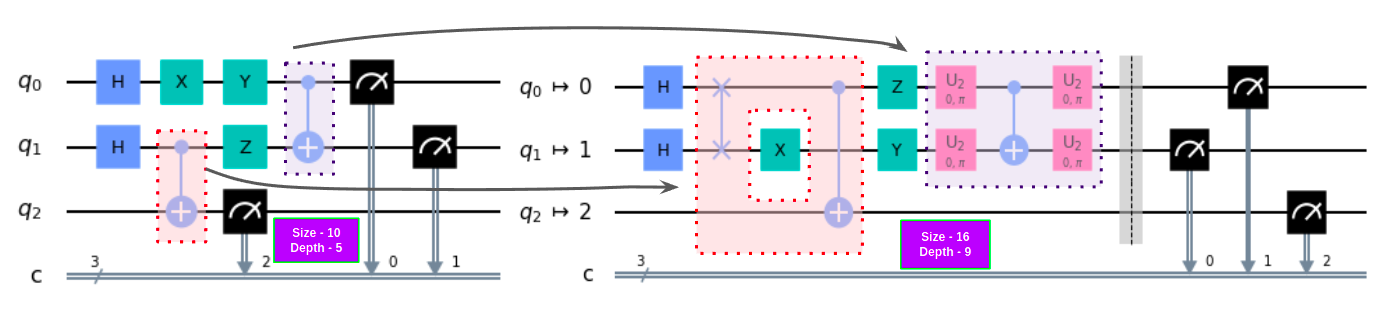
\includegraphics[width=\linewidth]{figures/intro/routing-transform.png}
    \caption{Transformation of a Quantum Circuit where non-local operations are scheduled to one implementable on the hardware (qubits 1 and 2 are not a local pair, 0 and 1, and 0 and 2 are). The decomposition of some gates is shown with arrows.}
    \label{fig:intro-qubit-routing-example}
\end{figure}

While solving the problem of routing, we note that the value of the entire set of actions scheduled at each timestep is largely dependent on the independent value of actions in the set, and the values added by the co-occurrance of small subsets of these actions, i.e. operations occuring on qubits significantly separated on hardware do not affect each other. This strikes a remarkable similarity with the general problem of search in combinatorial spaces \cite{qroute_dqn1}, an improvement in the solution to the routing problem with imply a new method to decide over subsets, as will an improvement in decision over subsets most likely imply an improvement in our router.

Annealers with Dense neural networks as proposed in \cite{qroute_dqn1,qroute_dqn2} were the only previous works which solve qubit routing phrased as a decision over sets problems. We noted the following challenges while running replications of both these results:
\begin{enumerate}
    \item\label{item:why-qroute-noise} Backpropagating rewards across the annealers is noisy, the combining algorithm needs to be a more deterministic function of it's inputs.
    \item\label{item:why-qroute-policy} Value function is hard to estimate, particularly in large circuits, since it requires massive forsight of how long it will take to schedule the rest of the circuit, while optimal actions can be chosen from a very shallow look ahead.
    \item\label{item:why-qroute-speed} Annealers are slow in high-value set construction and are infeasibly slow with a large number of qubits or gates.
    \item\label{item:why-qroute-horizon} The simulations need to be run on very long event horizons, however most of the actions should affect rewards in the near future. 
    \item\label{item:why-qroute-symmetries} The value function should model the symmetries inherent to the system and understand that swap actions chosen are only dependent on the local structure around the qubit.
\end{enumerate}

Over the past few years, reinforcement learning has shown remarkable breakthroughs in playing games like Go\cite{mcts-alphago}, Chess\cite{mcts-alphazero} using planning with Monte Carlo Tree Search, playing StarCraft\cite{rl-alphastar-blog} and Dota\cite{rl-openai-dota} using an actor critic method with combinatorial decisions for all agents taken using an actor-critic method trained in an autoregressive setting. These games are faced with tasks similar to those listed above, with long horizons to reason over, combinatorial search spaces requiring the coordination of many controlled agents, etc. being major issues. The fact that the methods used to solve these games are able to cope with these challenged motivated us to try them on the problem of routing as well.

Challenge \ref{item:why-qroute-noise} is well handled by using MCTS instead of the annealer setting. A value network and a policy network are used, which helps neurally prune the tree helping with challenge \ref{item:why-qroute-speed}, and the ability to model the policy directly in the policy network and training it in an actor critic setting solve challenge \ref{item:why-qroute-policy}. Greedy gate scheduling and intermediate rewards on each step as gates are scheduled helps avoid long-horizon reasoning, affressing challenge \ref{item:why-qroute-horizon}. The Graph Neural Network with a small number of message passing rounds models symmetries and localities well solving \ref{item:why-qroute-symmetries}.

Following the publication of our work, Zhou et. al. \cite{qroute_mcts} have proposed a similar MCTS-based method (without a neural guide) for depth minimization. This method shows promising results amongst other classical planners and heuristic methods, and shows that the choice of setting is valid even independent of the Machine Learning problem. Our method, however, is capable of routing larger circuits with better speed and lower depth.

\subsection{qLEET: Variational Circuit Property Visualizations}

Variational Methods (discussed in section \ref{sec:variational-circuits}) approach optimization problems, i.e. maximization or minimization under constraints, by posing them as the task of finding the ground state eigenvector of a hamiltonian which models the problem. The ground state is generated by a parametrized quantum circuit with guessed parameters, and the guess by a classical system.

Depending on the algorithm we use, the problem Hamiltonian as a function of the parameters of our prepared state can be easy or hard to optimize over. In classical machine learning, we have seen that model architecture, which is essentially the way the model is parametrized can affect the loss landscape it's optimizing over, and models which result in smooth landscapes perform well and those which do not show inferior results. The most striking of these demonstrations is by \cite{loss-landscapes}, as demonstrated in the image \ref{fig:loss-landscape-neural-nets}. 

\begin{figure}[ht]
    \centering
    \hfill
    \begin{subfigure}[b]{0.45\linewidth}
        \centering
        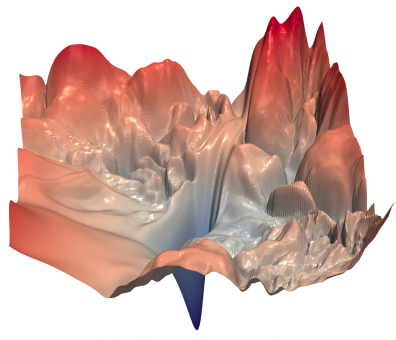
\includegraphics[width=0.7\textwidth]{figures/intro/landscape-rough.png}
        \caption{Loss Landscape without Skip Connections\label{fig:loss-landscape-rough}}
    \end{subfigure}
    \hfill
    \begin{subfigure}[b]{0.45\linewidth}
        \centering
        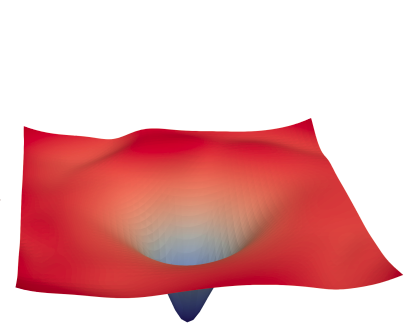
\includegraphics[width=0.7\textwidth]{figures/intro/landscape-smooth.png}
        \caption{Loss Landscape with Skip Connections\label{fig:loss-landscape-smooth}}
    \end{subfigure}
    \hfill
    \caption{The loss landscapes of neural networks with and without skip connections, as visualized by Li et. al.\cite{loss-landscapes}. The architectural decision of adding skip connections makes the feasibility of the optimization process a lot higher, to the extent visualizable on a 2-D random projection.}
    \label{fig:loss-landscape-neural-nets}
\end{figure}

In case the landscape we are optimizing over is not smooth, the optimization process is easily affected by the choice of initial variables. Furthermore, the convergence of differently initialized optimization runs, or lack thereof, tells us about the degree of abundance of local minima on this landscape. One notable example of such analysis is by Lorch \cite{training-trajectories}. We hope that by using similar analysis on parametrized quantum circuits, we can compute which class of circuits lead to better optimizability over the underlying hamiltonian. We give example analysis of this method on circuits like QAOA for computing the Max-Cut of a graph (formulation discussed in \ref{sec:variational-circuits-qaoa}) amonst others.

Furthermore, given that we are leveraging quantum computers to solve these problems, in addition to the optimization over the loss landscape we also need to ensure that these quantum resources are being efficiently utilized. For this, Sim et. al. \cite{expressibility-entanglability-guzik} have come up with two metric, expressibility and entanglement capability. 
\begin{itemize}
    \item The parametrization of the Variational Circuits affects what set of states it can generate, there can always exist some set of states which are not generatable by our parametrized anstaz for any choice of the parameter-vector. The amount of the state space that our circuit can generate is measured using the metric of expressibility, the higher the expressibility of the circuit, the better it is as exploring the entire space of solutions.  
    \item The quantum speedup in these variational circuits is attributed to entanglement between the qubits (discussed in section \ref{sec:background-unitary-gate-entanglement}), due to which the information being processed inside of the quantum circuit is exponentially greater than that which would have been by a classical system with the same number of qubits. A measure of how much of this entanglement capability is used by our PQC is a valuable metric, it's presence seems essential to 
\end{itemize}

In our PQC analysis software qLEET, build a backend agnostic suite of python packages which help evaluate this metric for well known variational algorithms like QAOA for Max-Cut on a Graph, Variational Quantum Eigensolvers, and the like. We include support for doing these evaluations on ideal conditions with pure state-vectors, or with density matrices and noise models. The final evaluation can be computed by sampling the quantum state, or by mathematically evaluating these metrics by accessing the underlying quantum state directly to speed up the computation.

\section{Thesis Layout}

\begin{itemize}
    \item[C1] This is the introductory chapter, which discusses the scope of the work carried out in this thesis in the context of developments in quantum computation, addresses the problems we are attempting to pose solutions to, and adds some motivation for the methods that we will develop in the following chapters.
    \item[C2] Here we presents a background in Quantum Computing and Reinforcement Learning which is requisite for understanding the motivations of the methods developed and the algorithms used in the remainder of this dissertation. We conclude this chapter by enlisting some ideas that we are going to use to address the problems posed in \ref{enum:problems-addressed-by-thesis}.
    \item[C3] As the first major contribution of this thesis, we present \textbf{qRoute: Qubit Routing using Graph Neural Network aided Monte Carlo Tree Search}, which is a reinforcement learning algorithm we propose for depth-minimized (used as a proxy for noise-mitigated) compilation. We discuss the problem of routing problem, discuss the specifics of our algorithm and associated neural architecture design.
    \item[C4] The other contribution of this thesis is \textbf{qLEET: Visualizing Loss Landscapes, Expressibility, Entangling power and Training Trajectories for Parameterized Quantum Circuits}, in which we present a way to analyze the properties of variational methods that can be implemented on present day quantum computers, and build a software framework for the same.
    \item[C5] We conclude with a summary of methods and results discussed in this thesis, the practical use-cases of these methods, and the scope of extension of this work in the future.
\end{itemize}

